\section{Parallelization performance}
\label{sec:dsmc_parallelization_performance}

\section{Results for simple geometries}
\subsection{Flow in a cylinder, varying Knudsen number}
We have induced flow in a voxelized cylinder as shown in figure \ref{fig:cylinder_flow}. The cylinder has radius $0.45 \mu m$ with an applied acceleration corresponding to a pressure difference $\Delta P = 1.1P_0$, where $P_0$ is the ideal gas pressure at $T=300K$. We can choose the Knudsen number through the density
\begin{align}
	\rho_n(\text{Kn}) = {1\over \sqrt 2 \pi d^2 \text{Kn}L},
\end{align}
where $L$ is the length of the cylinder. 

\begin{figure}[h]
\begin{center}
\includegraphics[width=\textwidth, trim=0cm 0cm 0cm 0cm, clip]{DSMC/figures/cylinder.png}
\label{fig:cylinder_flow}
\end{center}
\caption{Voxelized (128x128x128 voxels) cylinder with radius $0.45\mu m$.}
\end{figure}
We expect an apparent permeability following the Knudsen correction factor $f_c$ from section \ref{sec:knudsen_correction}
\begin{align}
	k_a = k_\infty f_c = k_\infty[1 + \alpha(\text{Kn})\text{Kn}]\left[1 + {4\text{Kn}\over 1 - b\text{Kn}}\right],
\end{align}
where $k_\infty$ is the high density limit permeability; the absolute permeability. The analytical absolute permeability for a cylinder is given by\cite{karniadakis2005microflows}
\begin{align}
	\label{eq:permeability_cylinder}
	k_\infty = {r^2\over 8},
\end{align}
which gives the following prediction for the apparent permeability
\begin{align}
	k_a = [1 + \alpha(\text{Kn})\text{Kn}]\left[1 + {4\text{Kn}\over 1 - b\text{Kn}}\right] {r^2\over 8}.
\end{align}
In figure \ref{fig:one_cylinder_varying_knudsen} we have plotted the measured permeability as a function of Knudsen number. We see that the permeability is slightly smaller than the analytical prediction as we would expect since the cylinder is voxelized.

\begin{figure}[h]
\begin{center}
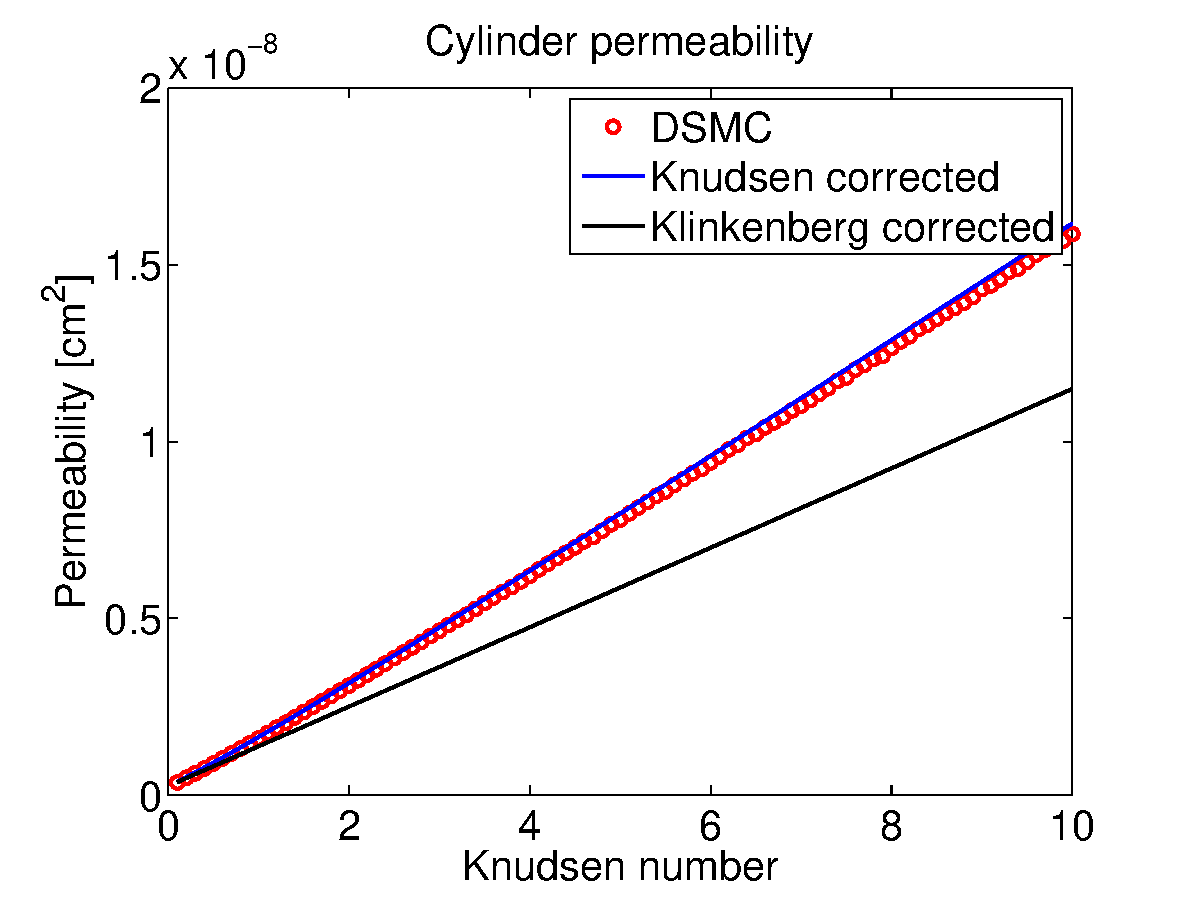
\includegraphics[width=\textwidth, trim=0cm 0cm 0cm 0cm, clip]{DSMC/figures/cylinder_knudsen_permeability.eps}
\label{fig:one_cylinder_varying_knudsen}
\end{center}
\caption{Permeability as a function of Knudsen number for a cylinder with radius $0.45 \mu m$ with an applied pressure difference $\Delta P = 1.1P_0$. The blue line is the Knudsen corrected analytical solution from \cite{karniadakis2005microflows}. The DSMC results show slightly higher permeability as we expect from the voxelation.}
\end{figure}

\subsection{Flow in a cylinder, varying radius}
If we instead keep the Knudsen number constant ($\text{Kn}=1.0$), we can vary the radius to verify equation \eqref{eq:permeability_cylinder}. We have studied radii in the range $0.1 \mu m$ to $0.45 \mu m$ with the same pressure difference as in the previous subsection. In figure \ref{fig:one_cylinder_varying_radii_result} we have plotted the measured permeability as a function of cylinder radius. The straight line confirms the quadratic dependency in equation \eqref{eq:permeability_cylinder}.
\begin{figure}[h]
\begin{center}
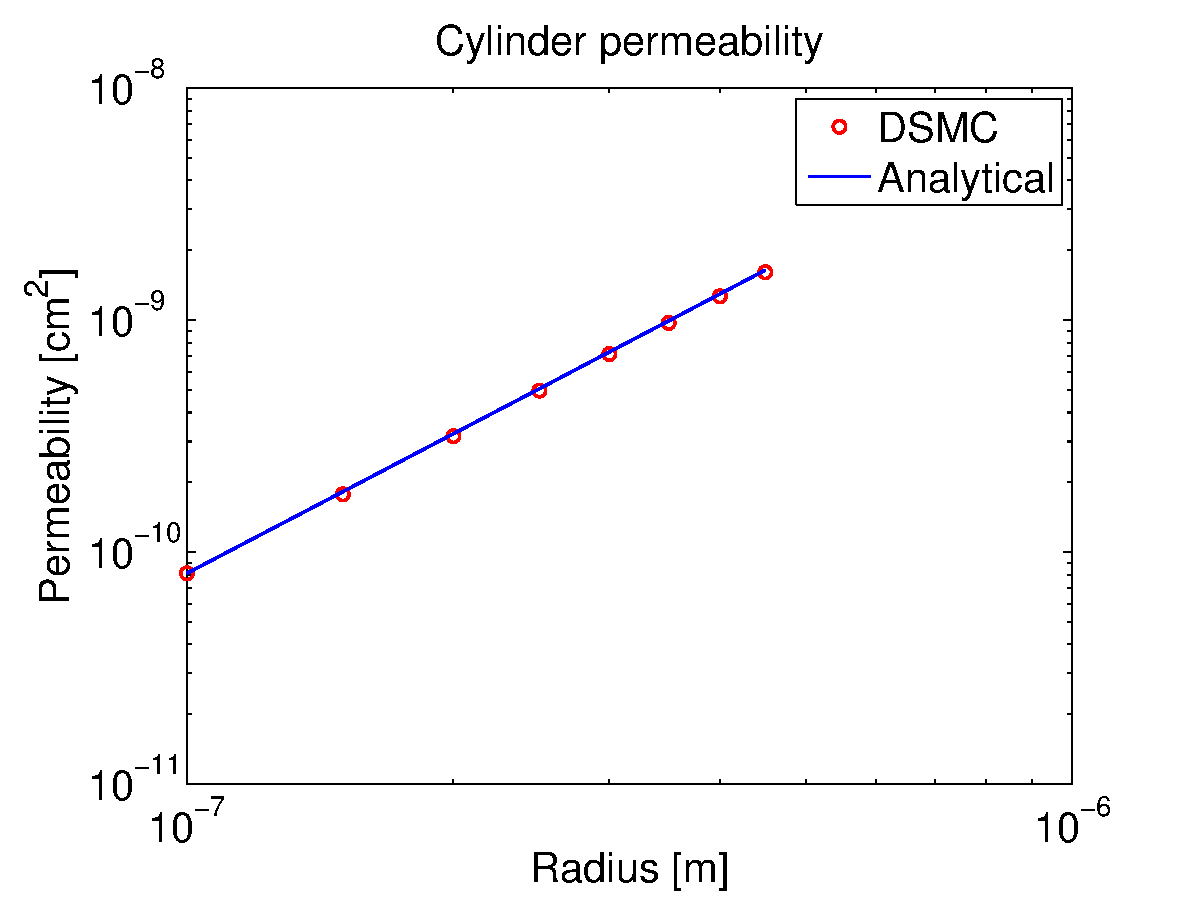
\includegraphics[width=\textwidth, trim=0cm 0cm 0cm 0cm, clip]{DSMC/figures/cylinder_radius_permeability.eps}
\label{fig:one_cylinder_varying_radii_result}
\end{center}
\caption{Logarithmic plot of the permeability for different cylinders with radii in the range $0.1 \mu m$ to $0.45 \mu m$ with an applied pressure difference $\Delta P = 1.1P_0$. The blue line is the Knudsen corrected analytical solution from \cite{karniadakis2005microflows}. The DSMC results show slightly higher permeability as we expect from the voxelation.}
\end{figure}
\section{Results for complicated geometries}
\subsection{Randomly packed spheres}
Through the Carman-Kozeny equation, we can theoretically predict the permeability for randomly packed spheres 
\begin{align}
	k = {a^2 \over 9K} {\phi^3 \over (1 - \phi)^2},
\end{align}
where $\phi$ is the porosity, $a$ is the sphere radius and $K$ Kozeny constant which is experimentally measured to be around five\cite{carman1937fluid}. This theoretical result has been verified to predict permeabilities in experiments, but at micrometer scale, we expect deviations. 
